\documentclass[12pt,a4paper]{article}

\usepackage{t1enc}
\usepackage[utf8]{inputenc}
\usepackage[magyar]{babel}
\usepackage{enumitem}
\usepackage[version=4]{mhchem}
\usepackage{xspace}
\usepackage{hyperref}
\usepackage{graphicx}
\usepackage{listings}
\usepackage{tabu}
\usepackage{makecell}
\usepackage{enumitem}

\graphicspath{ {./images/} }

\newcommand{\xml}{\textit{XML}\xspace}

\lstset{showstringspaces=false}
\lstset{ literate={á}{{\'a}}1 {é}{{\'e}}1 {í}{{{\'\i}}}1 {ó}{{\'o}}1 {ö}{{\"o}}1 {ő}{{\H o}}1 {ú}{{\'u}}1 {Ú}{{\'U}}1 {ü}{{\"u}}1 {ű}{{\H u}}1 {Ü}{{\"U}}1 }

\title{Android oktatóalkalmazás Java programnyelvhez}
\author{Gáspár Tamás}

\begin{document}
	
	%FŐOLDAL ------------------------------------------------------------------
	
	%intézet
	\thispagestyle{empty}
	\centerline{\textsc{\Large{Szegedi Tudományegyetem}}}
	\vspace{0.3 cm}
	\centerline{\textsc{\Large{Természettudományi és Informatikai Kar}}}
	
	\vspace*{2 cm}
	
	\centerline{\textsc{\Large{Informatikai Intézet}}}
	\vspace{0.3 cm}
	\centerline{\textsc{\Large{Számítógépes Optimalizálás Tanszék (?)}}}
	
	\vspace{3 cm}
	
	%cím
	\centerline{\LARGE{Android oktatóalkalmazás Java programnyelvhez}}
	\vspace{0.5 cm}
	\centerline{\Large{\textsc{Diplomamunka}}}
	
	\vspace{3 cm}
	
	\begin{flushleft}
		Készítette: Gáspár Tamás \newline
		Programtervező Informatikus MSc hallgató
	\end{flushleft}

	\vspace{1 cm}

	\begin{flushright}
		\hspace*{\fill} Témavezető: Dr. Csendes Tibor \newline
		\hspace*{\fill} Egyetemi tanár \newline
		\hspace*{\fill} Számítógépes Optimalizálás Tanszék 
	\end{flushright}
	
	\vspace{3 cm}
	
	\centerline{\Large{\textsc{Szeged, 2021}}}
	
	%tartalomjegyzék oldala -------------------------------------------------
	\newpage
	\thispagestyle{empty}
	
	\tableofcontents
	
	%tényleges kezdet --------------------------------------------------------
	\newpage
	\setcounter{page}{1}
	\fontsize{12}{16}\selectfont
	
	\section{Bevezető}

	...

	\section{A diplomamunka célja}
	
	A cél egy olyan Android eszközökön futó alkalmazás, ami segítséget nyújt a \textit{Java} programozási nyelv megtanulásához. Ehhez két komponensre van szükség: a konkrét alkalmazásra, mely képes valamilyen standard formában megadott tananyagot megjeleníteni, és magára a tananyagra.

	\subsection{Követelmények a tananyaggal kapcsolatban}
	
	A tananyagnak strukturáltnak kell lennie, hogy a felhasználó könnyen tudjon navigálni benne. A programozás alapjaitól kell kezdődnie, hogy teljesen kezdők számára is használható lehessen. Fontos, hogy a tananyag csak olyan ismeretekre hivatkozzon, amik már a korábbi fejezetekben be lettek mutatva. Lenniük kell számonkéréseknek is, amelyekkel a felhasználó megbizonyosodhat róla, hogy megértette-e az anyagot. 

	\subsection{Az alkalmazás követelményei}
	
	Az alkalmazásnak képesnek kell lennie, hogy a tananyagot a struktúráját megőrizve megjelenítse. A programozás oktatásánál elengedhetetlenek a kódminták, ezeket formázottan és könnyen olvashatóan kell mutatni (tabulálás, színezés). A felhasználó által kitöltött számonkéréseket ki kell tudni értékelni, a helyes és helytelen válaszokat pedig jelölni.
	
	\section{A tananyag struktúrája}  
	
	A tananyagot kurzusokra, fejezetekre, feladatokra és vizsgákra osztottam. A következő alfejezetekben részletesen leírom, hogy ezek mit takarnak.
		
	\subsection{XML}
	
	Az \xml (\textit{Extensible Markup Language}) egy jelölőnyelv, ami alkalmas strukturált adattárolásra. Az \xml fájlok egymásba ágyazott \textit{tag}ekbből állnak. Egy példa \xml-ben megadott adatra, ami egy azonosító és egy név \textit{tag}et tartalmaz:
	
	\begin{lstlisting}[language=XML]
<root>
  <id>33</id>
  <name>XML</name>
</root>
	\end{lstlisting}
	
	A beépített \textit{Android} erőforrástípusok \xml-t használnak, ezért számomra is természetes volt, hogy ebben kódolom el a tananyag erőforrásfájljait.
	
	A továbbiakban az \xml dokumentumokban azokat a részeket, ahol nem konkrét adatot kell érteni [ és ] jelek közé fogom írni, ezáltal általánosabban adhatom meg a struktúrákat. A fenti \xml így átírva:
	
	\begin{lstlisting}[language=XML]
<root>
  <id>[Azonosító]</id>
  <name>[Név]</name>
</root>
	\end{lstlisting}
	
	\subsection{Kurzus}
	
	A kurzus a legnagyobb egység, a \textit{Java} nyelv egy nagy területéhez kapcsolódó ismereteket tartalmazza. Ezek az ismeretek lehetnek egyszerűek (a tananyag elején), vagy magas szintűek, amelyek már a korábbi kurzusokra épülnek (jellemzően a későbbi kurzusok).
	
	Külön kurzusba vettem például az adatszerkezeteket, vagy a generikus programozást. Természetesen ezek a területek önmagukban is rengeteg ismeretet tartalmaznak, ezért további felosztásra van szükség, ezért bevezettem a fejezeteket.
	
	Minden kurzus tartalmaz egy nevet és egy egyedi azonosítószámot, méghozzá úgy, hogy ezek a számok növekvő sorrendbe állítva meghatározzák a kurzusok sorrendjét.
	
	Ezen kívül minden kurzus tartalmazza, hogy mely fejezetek (\ref{fejezet}), feladatok (\ref{feladat}) és vizsga (\ref{vizsga}) tartozik hozzájuk.
	
	A fentiek alapján egy kurzust leíró \xml fájl a következőképpen néz ki:
	
	\begin{lstlisting}[language=XML]
<resources>
  <coursedata>
    <id>[Kurzus azonosító]</id>
    <name>[Kurzusnév]</name>
    <finished>[Befejezettség jelölő]</finished>
  </coursedata>
  
  <chapter>[Fejezet azonosító]</chapter>
  ...
  <chapter>[Fejezet azonosító]</chapter>
  
  <task>[Feladat azonosító]</task>
  ...
  <task>[Feladat azonosító]</task>
  
  <exam>[Vizsga azonosító]</exam>
</resources>
	\end{lstlisting}
	
	Arról, hogy mit takar a befejezettség jelölő és a \textit{<finished>} tag, a \ref{reszben_befejezett_kurzusok} alfejezetben írok.
	
	\subsection{Fejezet}\label{fejezet}
	
	A kurzus nem osztatlan egység, hanem fejezetekből épül fel. Ezek további kisebb, összefüggő részekre bontják a kurzus tartalmát, hogy az átláthatóbb és könnyebben elsajátítható legyen.
	
	Például az adatszerkezetek kurzus fejezetei a következők:
	
	\begin{enumerate}
		\item Tömbök.
		\item A tömbök hátrányai.
		\item Listák.
		\item Verem és sor.
		\item Szótár.
		\item Hasznos osztályok adatszerkezetek kezelésére.
	\end{enumerate}  

	A listából látszik, hogy vannak átkötő fejezetek is, melyek elmagyarázzák, hogy miért fontosak a korábbi, vagy későbbi fejezetek ismeretei. Például a \textit{Tömbök} fejezet után a felhasználóban felmerülhet, hogy miért kell további adatszerkezetekkel foglalkozni. Ezért közbeiktattam egy plusz fejezetet, ami részletesen megmagyarázza, hogy milyen hátrányai vannak a tömböknek és hogy mely esetekben érdemes más adatstruktúrát választani.
	
	A fejezetek is rendelkeznek azonosítóval és névvel. Ezen kívül tartalmazzák a fejezet törzsét, ami majd konkrétan megjelenik a felhasználónak, amikor megnyitja az adott fejezetet. 
	
	\begin{lstlisting}[language=XML]
<resources>
  <chapterdata>
	<id>[Fejezet azonosító]</id>
    <name>[Fejezetnév]</name>
  </chapterdata>

  [Fejezet törzse]	
	
</resources>
	\end{lstlisting}
	
	Arról, hogy mi tartozhat a törzsbe, és ezek hogyan vannak elkódolva, a \ref{torzs_kodmintak_kerdesek}. részben írok részletesen.
	
	\subsection{Feladat}\label{feladat}
	
	A feladat egy önálló programozási munkát takar, ami mindig egy kurzushoz kapcsolódik. Ahhoz, hogy a felhasználó meg tudja oldani, szüksége lesz az adott kurzus és az azt megelőző kurzusok ismereteire is.
	
	Egy kurzushoz több feladat is tartozhat, de mindegyikhez adott legalább egy. Továbbra is maradva az adatszerkezetek kurzusnál, ehhez például két feladatot mellékeltem:
	
	\begin{itemize}
		\item Tömb alapú lista implementálása.
		\item Láncolt lista implementálása.
	\end{itemize}

	Megjegyzem, hogy ezen feladatok megoldásának nem kell olyan hatékonynak vagy általánosnak lennie, mint egy valódi implementáció, a cél csak a két lista alapelveinek megértése. Mivel a generikus programozás kurzus az adatszerkezetek után következik, ezért itt természetesen nem elvárás generikus listák programozása.

	Egy-egy feladatnak olyan sokféle helyes implementációja van, hogy lehetetlen ellenőrizni, hogy a felhasználó megoldása megfelelő-e. Ennek ellenére szerettem volna biztosítani, hogy ha a felhasználó elakad, vagy csak összevetné a megoldását egy másikkal, akkor erre lehetősége legyen. Minden feladat mellé referencia implementációt mellékeltem, ami az adott feladat alatt megtekinthető.

	A feladatok \xml elkódolása így néz ki:
	
	\begin{lstlisting}[language=XML]
<resources>
  <taskdata>
    <id>[Feladat azonosító]</id>
    <name>[Feladatnév]</name>
  </taskdata>
  
  [Feladat törzs]
  	
  <solution>
  
  [Referencia implementáció törzs]
  
  </solution>
</resources>
	\end{lstlisting}

	Arról, hogy mi tartozhat a törzsbe, és ezek hogyan vannak elkódolva, a \ref{torzs_kodmintak_kerdesek}. részben írok részletesen.

	\subsection{Vizsga}\label{vizsga}
	
	A vizsgák a tananyag valódi számonkérései, itt ugyanis a feladatokkal ellentétben lehetséges a megoldások pontos ellenőrzése. Minden kurzushoz egy vizsga tartozik, amelyben benne lehet bármi az adott kurzus fejezeteiből.
	
	Azért, hogy az alkalmazás a válaszokat ellenőrizni tudja, megkötéseket kell tenni a kérdések típusára. Nem lehet például esszékérdés. Ezt figyelembe véve a következő kérdéstípusokat implementáltam:
	
	\begin{itemize}
		\item Feleletválasztós kérdés, egy választási lehetőséggel (\textit{single choice}).
		\item Feleletválasztós kérdés, több választási lehetőséggel (\textit{multi choice}).
		\item Szöveges kérdés, ahol a válasz egy szó vagy rövid kifejezés lehet.
		\item Igaz-hamis kérdés.
	\end{itemize}
	
	A vizsgákhoz kérdéshalmaz tartozik, melyből az alkalmazás véletlenszerűen választ annyi, amennyi kérdésből az adott vizsga áll (jellemzően 25-30 darabot). Időlimit is van, ami alatt a felhasználónak be kell fejeznie a kitöltést. Az idő lejárta esetén a kitöltés akkori állapota kerül kiértékelésre.
	
	Sikeres vizsga esetén a következő kurzus elérhetővé válik. Amennyiben a vizsga nem sikeres, akkor néhány óráig nem lesz újra kitölthető. Ezt a korlátozást azért vezettem be, hogy ne lehessen a vizsgákat "\textit{brute-force}" módon teljesíteni. Ha a felhasználó már korábban sikeresen elvégezte a vizsgát, akkor azt korlátozás nélkül bármikor újra elindíthatja. A vizsgán elért legmagasabb pontszám eltárolásra kerül.
	
	A vizsgákat definiáló \xml fájlok a következőképpen néznek ki:
	
	\begin{lstlisting}[language=XML]
<resources>
  <examdata>
	<id>[Vizsga azonosító]</id>
	<questionAmount>[Kérdések mennyisége]</questionAmount>
	<timeLimit>[Időkorlát, perceben]</timeLimit>
    <finished>[Befejezettség jelölő]</finished>
  </examdata>
  
  [Vizsgakérdések]
  
</resources>
	\end{lstlisting}

	Arról, hogy mit takar a befejezettség jelölő és a \textit{<finished>} tag, a \ref{reszben_befejezett_kurzusok}. alfejezetben írok. A kérdéstípusok részletes definiálása a \ref{kerdesek}. részben történik.
	
	\subsection{Előrehaladás a tananyagban}
	
	Az alkalmazás kezdeti indításakor a felhasználó csak az első kurzus fejezeteihez és feladataihoz fér hozzá. A vizsga zárolva van. El kell olvasnia az összes fejezetet ahhoz, hogy a vizsga kitölthető legyen. A feladatok elkészítése opcionális, de ajánlott.
	
	A vizsga sikeres teljesítésével nyitható meg a következő kurzus, majd a folyamat ismétlődik addig, amíg van további kurzus.
	
	Korábbi fejezetek, feladatok, és vizsgák bármikor újra megtekinthetőek és kitöltetőek. 
	
	\subsection{Részben befejezett kurzusok}\label{reszben_befejezett_kurzusok}
	
	\section{Törzstartalom, kódminták és kérdések}\label{torzs_kodmintak_kerdesek}
	
	Már láttuk a tananyag struktúráját és azt, hogy ez hogyan van \xml-ben elkódolva. Most bemutatom, hogy miként vannak definiálva azok a komponensek, amelyeket a felhasználó a fejezetek, feladatok és vizsgák megnyitásakor lát és amelyek a tananyag törzsét alkotják.
	
	\subsection{Szöveges tartalmak}
	
	Egyszerű szöveg és cím tag leírása ide.
	
	\subsubsection{Bekeretezett szöveg}
	
	...
	
	\subsubsection{Magas szintű tartalom}
	
	...
	
	\subsection{Grafikus tartalmak}
	
	Kép beillesztés leírása ide.
	
	\subsection{Kódminták}
	
	...
	
	
	\subsection{Interaktív kódminták}
	
	...
	
	
	\subsection{Kérdések}\label{kerdesek}
	
	...
	
	\subsubsection{feleletválaszós kérdés egy válaszlehetőséggel}
	
	...
	
	\subsubsection{feleletválaszós kérdés több válaszlehetőséggel}
	
	...
	
	\subsubsection{Szöveges kérdés}
	
	...
	
	\subsubsection{Igaz-hamis kérdés}
	
	...
	
	\section{A tananyag tárolása}\label{tananyag_tarolasa}
	
	A tananyagot a forráskódtól el kell különíteni, viszont futásidőben elérhetőnek kell lennie, hogy a felhasználó kéréseit ki lehessen szolgálni. Fontos az egységes elkódolás. Például minden kurzust leíró erőforrásfájlnak azonos felépítésűnek kell lennie: meg kell mondaniuk mely fejezetek, feladatok és vizsga tartozik hozzájuk.
	
	\subsection{Android erőforráskezelés}
	
	Az \textit{Android} alapelve, hogy az erőforrásfájlok legyenek elkülönítve a kódtól, és erre több eszközt is kínál. Az első a \textit{Resource System}. Ebben olyan erőforrásfájlok tárolhatóak, melyekre a legtöbb alkalmazásnak szüksége van:
	
	\begin{itemize}
		\item Grafikus elemek (\textit{drawable}): lehetnek ikonok, képek, hátterek, stb.
		\item Szövegek (\textit{string}): a felhasználói felületen megjelenő feliratok.
		\item Elrendezések (\textit{layout}): a felhasználói felület elrendezését tárolják.
		\item Még sok további előre definiált kategória: stílusok, színek, stb.
	\end{itemize} 

	A \textit{Resource System} nem a legmegfelelőbb mód a tananyag tárolására, mivel az egyetlen gyakori, előre definiált kategóriába sem esik. 
	
	Biztosított továbbá az \textit{Asset System}, mely annyiban tér el az előbb bemutatott rendszertől, hogy itt nincsenek kategóriák, be tud fogadni bármilyen erőforrásfájlt, amelyre egy alkalmazásnak szüksége lehet. Ez a legalkalmasabb módszer a tananyag tárolására.
	
	\section{Adatbázis}
	
	Az alkalmazásnak képesnek kell lennie eltárolnia felhasználó előrehaladását a tananyagban. A következő adatokat kell elmenteni:
	
	\begin{itemize}
		\item Teljesített vizsgák: Ez az információ a legfontosabb, mivel meghatározza, hogy melyik kurzusok elérhetőek.
		\item Elolvasott fejezetek: Mivel egy kurzus vizsgája csak akkor nyílik meg, ha a felhasználó minden fejezetet elolvas az adott kurzusból.
		\item Teljesített feladat: A feladatok teljesítése opcionális, de az alkalmazás ezt is eltárolja.
	\end{itemize}
	
	A \ref{tananyag_tarolasa} fejezetben említett \textit{Resource System} és \textit{Asset System} futásidőben csakis fájl olvasást tesznek lehetővé, írást nem. Ezért egy relációs adatbázist használok. \textit{NoSQL} adatbázis is lehetne, arról hogy miért a választott módszer mellett döntöttem, a \ref{sqlite_roon} fejezetben írok.
	 
	\subsection{Státusz annotáció}\label{statusz}
	
	Az előrehaladást a programban és az adatbázisban is egységesen jelölöm. Erre egy saját \textit{Java} annotációt használok:
	
	\begin{lstlisting}[language=Java]
@IntDef
public @interface Status {

	int LOCKED = 0;
		
	int UNLOCKED = 1;
		
	int COMPLETED = 2;
}
	\end{lstlisting}
	
	Az \textit{@IntDef} annotáció listázza, hogy mik lehetnek a lehetséges értékei egy olyan változónak, melyek \textit{@Status} annotációval látunk el. Ez fordítási időben ellenőrzésre kerül. Például ha a felhasználó először teljesít egy vizsgát, akkor annak státusza \textit{UNLOCKED}-ról \textit{COMPLETED}-re for változni az adatbázisban.
	 
	\subsection{Struktúra}
	 
	Az adatbázis szerkezete egyszerű. A tananyag négy egységéhez (kurzus, fejezete, feladat, vizsga) rendel egy-egy táblát, és ezen táblák rekordjai tárolják az előrehaladást. Így néz ki az egyed-kapcsolat diagram:
	
	\begin{center}
		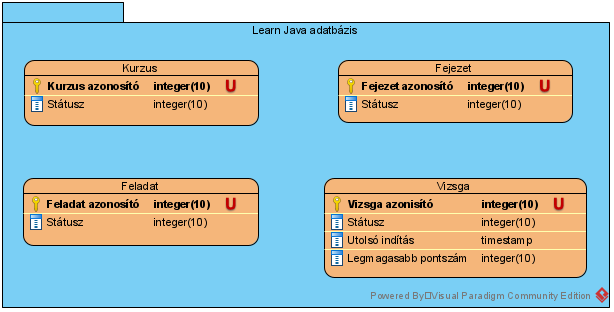
\includegraphics[width=\linewidth]{db_model}
	\end{center}
	
	Táblák közti kapcsolatra, külső kulcsokra nincs szükség. Az, hogy mely fejezetek és feladatok tartoznak egy-egy kurzushoz nem az adatbázisban van eltárolva, hanem a tananyagot definiáló \xml dokumentumokban (mivel nem változik dinamikusan).
	
	Az azonosítók megegyeznek az \xml dokumentumokban használt azonosítókkal. A státusz mezők mindig a \ref{statusz} részben definiált annotáció valamelyik értékét tartalmazzák.
	
	A vizsgák esetén vannak további dinamikusan változó adatok:
	
	\begin{itemize}
		\item Az utolsó indítás időpontja: Ez szükséges, hogy a \ref{vizsga} részben említett indítási korlátot be lehessen tartani.
		\item Legmagasabb pontszám: Dinamikusan változó, ezért az adatbázisban kell tárolni.
	\end{itemize}
	
	\subsection{Megvalósítás: SQLite és Room}\label{sqlite_roon}

	Az Android rendszer minden alkalmazás számára biztosít egy \textit{SQLite} relációs adatbázist. Számomra egyértelmű volt, hogy ezt fogom használni. Az \textit{SQLite} egy olyan adatbázis kezelő, amely nem kliens-szerver alapú, hanem közvetlenül az őt használó alkalmazásba van beágyazva. 
	
	Ennek előnye, hogy nem kell hálózati kapcsolat az adatbázis eléréséhez, és nem kell szervert üzemeltetni. Hátránya viszont, hogy minden adat lokálisan kerül eltárolásra. Ennél az alkalmazásnál ez nem jelent gondot, mivel viszonylag kevés rekord keletkezik (a tananyag minden eleméhez egy).
	
	Az alkalmazás saját adatbázisának közvetlenül is küldhetünk üzenetet, ez azonban több okból sem javasolt:
	
	\begin{itemize}
		\item Szintaktikus hibák: ha a kiadott \textit{SQL} utasításban szintaktikus hibát vétünk, az a program helytelen működéséhez, összeomlásához vezet. Ez nincs ellenőrizve.
		\item Érvénytelen utasítások: ha olyan utasítást adunk ki, amelyet az \textit{SQLite} nem tud végrehajtani, akkor is helytelen viselkedés fog történni. Például, ha olyan rekordot szúrunk be, ami sérti az egyediség feltételt.
		\item Adatbázis frissítés a főszálon: ha a főszálon adunk ki \textit{SQL} utasítást, akkor ez blokkolni fog, és a felhasználói felület nem lesz válaszképes. 
	\end{itemize}

	Pontos tervezéssel és helyes implementációval ez mind elkerülhető, de javasolt egy olyan keretrendszer használata, mely az adatbázis kezelés veszélyeit kezeli. Egy ilyen keretrendszer a \textit{Room}, amely az Android fejlesztői könyvtár (\textit{AndroidX}) része.
	
	A \textit{Room} elrejti a programozó elől az \textit{SQLite} adatbázist, helyette két komponenst biztosít, melyekkel a struktúrája és tartalma módosítható. Ezen kívül meg fogja tiltani, hogy a főszálról adatbázis műveletet végezzünk (ilyen esetben kivétel dobódik). 
	
	\subsubsection{Room entitások}
	
	Az entitások olyan \textit{@Entity} annotációval jelölt Java osztályok, melyek megadják az adatbázis tábláinak struktúráját. Például a fejezet táblát a következőképpen definiáltam:
	
	\begin{lstlisting}[language=Java]
@Entity(tableName = "chapter_status")
public class ChapterStatus {
	
 @PrimaryKey //külső kulcs jelző
 @ColumnInfo(name = "chapter_id")
 private int chapterId;
	
 @ColumnInfo(name = "status")
 @Status //saját státusz annotáció
 private int status;
 
 //konstruktor...
}
	\end{lstlisting}  
	
	Látható, hogy annotációk segítségével adhatjuk meg, hogy milyen mezői legyenek az adott táblának. Az alkalmazás indításakor ez a tábla létre fog jönni az adatbázisban, anélkül, hogy egyetlen \textit{SQL} utasítást is írnunk kellene. Azokat a \textit{Room} fogja összeállítani, az általunk megadott adatok alapján, és garantáltan helyesek lesznek.
	
	A későbbiekben ezt az osztályt példányosíthatjuk, ezek az objektumok rekordokat fognak reprezentálni.

	\subsubsection{Room adatkezelők}
	
	Az adatkezelő objektumok olyan \textit{@Dao} annotációval jelölt Java interfészek, amikkel az előző részben definiált táblák tartalmát módosíthatjuk. Például a fejezet táblához a következő módosító interfészt készítettem:
	
	\begin{lstlisting}[language=Java]
@Dao
public interface ChapterDao {
	
 @Insert //a beszúró SQL utasítás automatikusan generálódik
 void addChapterStatus(ChapterStatus chapterStatus);
	
 @Update //a frissítő SQL utasítás automatikusan generálódik
 void updateChapterStatus(ChapterStatus chapterStatus);
	
 @Query("SELECT * FROM chapter_status WHERE chapter_id == :chapterId")
 ChapterStatus queryChapterStatus(int chapterId);
}
	\end{lstlisting}

	Bizonyos egyszerű műveletekre vannak előre adott annotációk, melyek automatikusan fogják generálni a a megfelelő \textit{SQL} utasítást (beszúrás, frissítés, törlés). Ezek azonban nem elegendőek, ezért a \textit{@Query} annotációval saját utasítást írhatunk. Ennek a tartalma fordítási időben ellenőrizve lesz. Megfigyelhető, hogy még arra is lehetőség van, hogy a kapott paraméterek értékét behelyettesítsük az \textit{SQL} utasításba.

	Egy példa arra, hogy hogyan kombinálhatjuk ezeket az osztályokat az adatbázis módosítására:
	
	\begin{lstlisting}[language=Java]
//egy új szálon
new Thread(() -> {
 ChapterDao dao = ... ;
 ChapterStatus cs = new ChapterStatus(id, Status.UNLOCKED);
 //beszúrás
 dao.addChapterStatus(cs);
}).start();
	\end{lstlisting}

\end{document}
